\subsection{Diagrammi dei package}
\subsubsection{Client side}
\begin{figure}[hb]
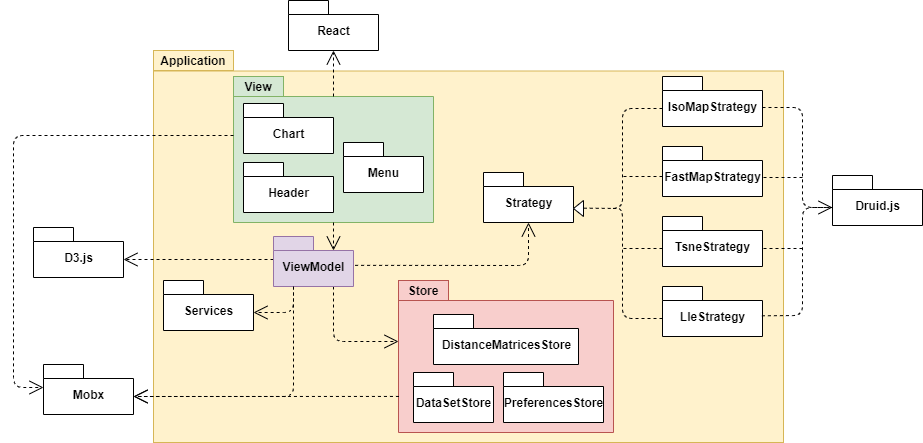
\includegraphics[width=18cm]{Images/Allegato Tecnico-Package}
\centering
\caption{Diagramma dei package client side}
\end{figure}

Il diagramma sopra riportato descrive a livello di package le parti che compongono il lato client dell'applicazione. In particolare si può notare che:
\begin{itemize}
	\item \textit{View} e \textit{Store} (ossia il modello) non siano direttamente collegati, ma il passaggio delle informazioni avviene solo attraverso un \textit{ViewModel}, unico per ciascun componente della vista che richieda una connessione allo store; 
		\item MobX ha il ruolo fondamentale di applicare il \glo{design pattern Observer}, ossia permette di rendere i dati contenuti nei vari store \glo{observable} e i componenti della vista che li utilizzano \glo{observer} (per esempio i grafici);
	\item Druid.js è importata solo nelle classi concrete degli algoritmi implementati (IsoMap, FastMap, Tsne, LLE) per eseguire la riduzione dimensionale e D3.js solo nei \textit{ViewModel} delle varie visualizzazioni (Scatterplot Matrix, HeatMap, Adjacency Matrix, Force Field, PLMA);
	\item La maggior parte delle dipendenze partono dai diversi \textit{ViewModel} verso le altri parti della web application, lasciando che la \textit{View} si occupi solo di ritornare le componenti che compongono la vista.
\end{itemize} 

\newpage
\subsubsection{Connessione tra client e server side}
\begin{figure}[hb]
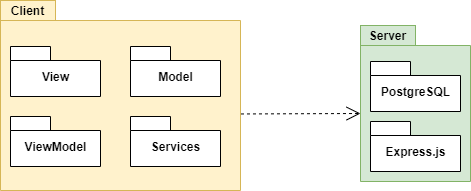
\includegraphics[width=12cm]{Images/Allegato Tecnico-Package 2}
\centering
\caption{Connessione tra client side e server side}
\end{figure}
La connessione tra client e server è così gestita:
\begin{itemize}
	\item Il server fornisce l'interfaccia per l'interrogazione del database attraverso delle API costruite con Express.js;
	\item Il client sfrutta \glo{Axios} per la connessione al server;
	\item Grazie ad alcune funzioni richiamate nel \textit{ViewModel} dedicato al caricamento dei dati dal database, vengono inviate le query di selezione al server che si occupa di interrogare il DB, il quale restituisce il risultato dell'interrogazione.
\end{itemize}